\documentclass[10pt, a4paper]{article}
\usepackage{cmap}
\usepackage[T2A]{fontenc}
\usepackage[utf8]{inputenc}
\usepackage[english, russian]{babel}
\usepackage[dvipsnames,table,xcdraw]{xcolor}
\usepackage{
	amsmath,
	amssymb,
	scrextend,
	enumitem,
	pscyr,
	multicol,
	cmap,
	titling,
	indentfirst,
	cancel,
	wrapfig,
	gensymb,
	tikz,
	graphicx,
	fancyhdr,
	mathrsfs,
	graphbox,
	indentfirst
}
%Параметры страницы
\usepackage[left=15mm,right=15mm,
top=2cm,bottom=2cm]{geometry}
\pagestyle{fancy}
%Путь к картинкам
\graphicspath{{pic/}}
\DeclareGraphicsExtensions{.pdf,.png,.jpg}
%Числа в списке второго уровня по умолчанию
\renewcommand{\labelenumii}{\arabic{enumii})}
%Новые команды
\newcommand{\answer}[1]{\textcolor[rgb]{0.8,0.8,0.8}{\fbox{#1}}}
\newcommand{\ranswer}[1]{\textcolor[rgb]{0.8,0.8,0.8}{\begin{flushright}\fbox{#1}\end{flushright}}}

%Русские символы в списке
\AddEnumerateCounter{\asbuk}{\russian@alph}{щ}

%Сеттеры
\setlength{\parindent}{5ex}
\setlength{\parskip}{1em}

\begin{document}
		
\lhead{Функции}
\rhead{Школа <<Симметрия>>}

\section{Линейная функция}
\begin{enumerate}
	\item Выяснить, лежат ли точки $A(-2;-2)$, $B(10;4)$ и $C(17;10)$ на одной прямой. \ranswer{Нет}
	\item Выяснить, лежат ли точки $A(6;-6)$, $B(10;10)$ и $C(12;18)$ на одной прямой. \ranswer{Да}
	\item Выяснить, лежат ли точки $A(-11;6)$, $B(-6;3)$ и $C(4;-3)$ на одной прямой. \ranswer{Да}
	\item Выяснить, лежат ли точки $A(-11;6)$, $B(-6;3)$ и $C(9;-6)$ на одной прямой. \ranswer{Да}
	\item Выяснить, лежат ли точки $A(-11;6)$, $B(4;-5)$ и $C(-6;3)$ на одной прямой. \ranswer{Нет}
	\item Выяснить, можно ли через точки $A(-6;6)$, $B(2;-8)$, $C(-8;-2)$ и $D(14;-6)$ провести две параллельные линии. \ranswer{Да, можно}
	\item
	\begin{minipage}[t]{0.6\textwidth}
		Прямые $f(x)=x-5,5$ и $g(x)$ пересекаются в точке с координатами $(a;b)$. Найдите $a+b$.
		
		\ranswer{$-10$}
	\end{minipage}
	\begin{minipage}[t]{0.3\textwidth}
		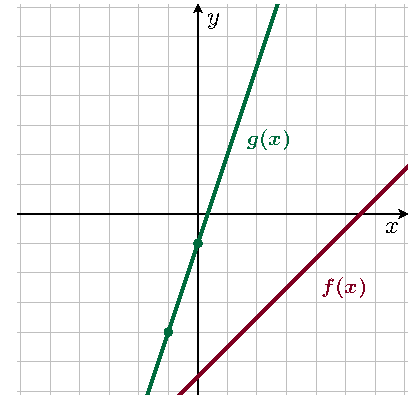
\includegraphics[align=t, width=\textwidth]{../graphs/graph_6/graph_6}
	\end{minipage}
	\item
	\begin{minipage}[t]{0.6\textwidth}
		Найдите координаты точки пересечения прямых $f(x)$ и $g(x)$. В ответ запишите сумму абсциссы и ординаты.
		
		\ranswer{$3,75$}
	\end{minipage}
	\begin{minipage}[t]{0.3\textwidth}
		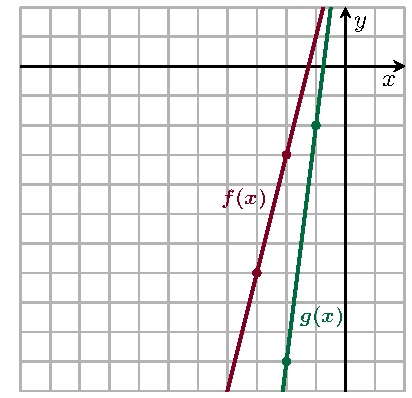
\includegraphics[align=t, width=\textwidth]{../graphs/graph_5/graph_5}
	\end{minipage}
\end{enumerate}
\section{Параболы}
\begin{enumerate}
	\item
	\begin{minipage}[t][8cm][t]{0.5\textwidth}
		На рисунке изображен график функции вида $y=ax^2+bx+c$, где числа $a$, $b$ и $c$ — целые. Вычислите $f\left(\dfrac{1}{4}\right)-f\left(\dfrac{1}{2}\right)$.
		\begin{flushright}
			\rotatebox{180}{\fbox{$-0,3125$}}
		\end{flushright}
	\end{minipage}
	\begin{minipage}[t][8cm][t]{0.5\textwidth}
		\hspace{10pt}
		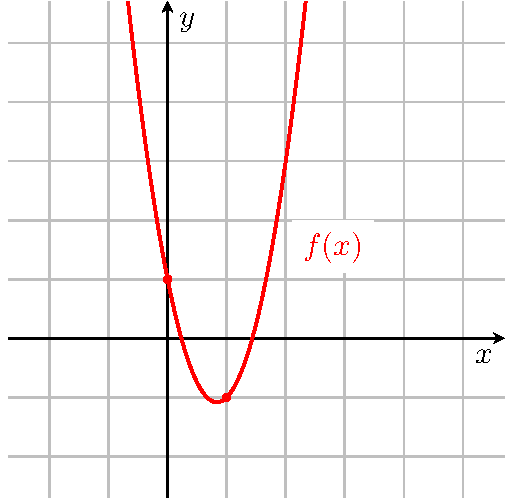
\includegraphics[align=t, width=0.8\textwidth]{graphs/graph_1/graph_1}
	\end{minipage}
\end{enumerate}
\section{Гиперболы}
\begin{enumerate}
	\item 
	\begin{minipage}[t][8cm][t]{0.5\textwidth}
		На рисунке изображен график функции вида $y=\dfrac{a}{x+b}+c$, где числа $a$, $b$ и $c$ — целые. Найдите $f\left(-\dfrac{8}{5}\right)$.
		\begin{flushright}
			\rotatebox{180}{\fbox{$-1\dfrac{1}{3}$}}
		\end{flushright}
	\end{minipage}
	\begin{minipage}[t][8cm][t]{0.5\textwidth}
		\hspace{10pt}
		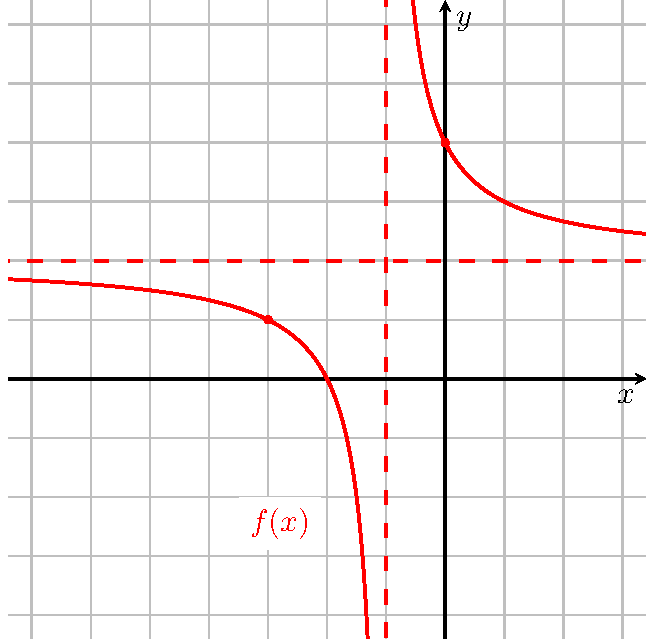
\includegraphics[align=t, width=0.8\textwidth]{graphs/graph_2/graph_2}
	\end{minipage}
	
\end{enumerate}
\end{document}